%%% Local Variables:
%%% TeX-command-extra-options: "-shell-escape"
%%% mode: latex
%%% TeX-master: t
%%% End:
\documentclass{beamer}
\usepackage{caption}
\usepackage{minted}
\usepackage{tikz}
\usepackage{xcolor}
\usetikzlibrary{shapes.geometric, arrows}
\tikzstyle{startstop} = [rectangle, rounded corners, minimum width=3cm, minimum height=1cm,text centered, draw=black, fill=red!30]
\tikzstyle{io} = [trapezium, trapezium left angle=70, trapezium right angle=110, minimum width=1.5cm, minimum height=0.6cm, text centered, draw=black, fill=blue!30]
\tikzstyle{process} = [rectangle, minimum width=1.5cm, minimum height=0.5cm, text centered, draw=black, fill=orange!30]
\tikzstyle{decision} = [circle, radius=2.5cm, text centered, draw=black, fill=green!30]
\tikzstyle{arrow} = [thick,->,>=stealth]
\usepackage[labelformat=simple]{subcaption}

\usetheme{Singapore}
\title{Abstraction}

\begin{document}
\begin{frame}
\titlepage
\end{frame}
\section{Abstract Nonsense}

\begin{frame}
  \huge \centering \url{https://en.wikipedia.org/wiki/Abstract_nonsense}
\end{frame}

\begin{frame}
  \frametitle{Software Engineers and Patterns}
  \centering 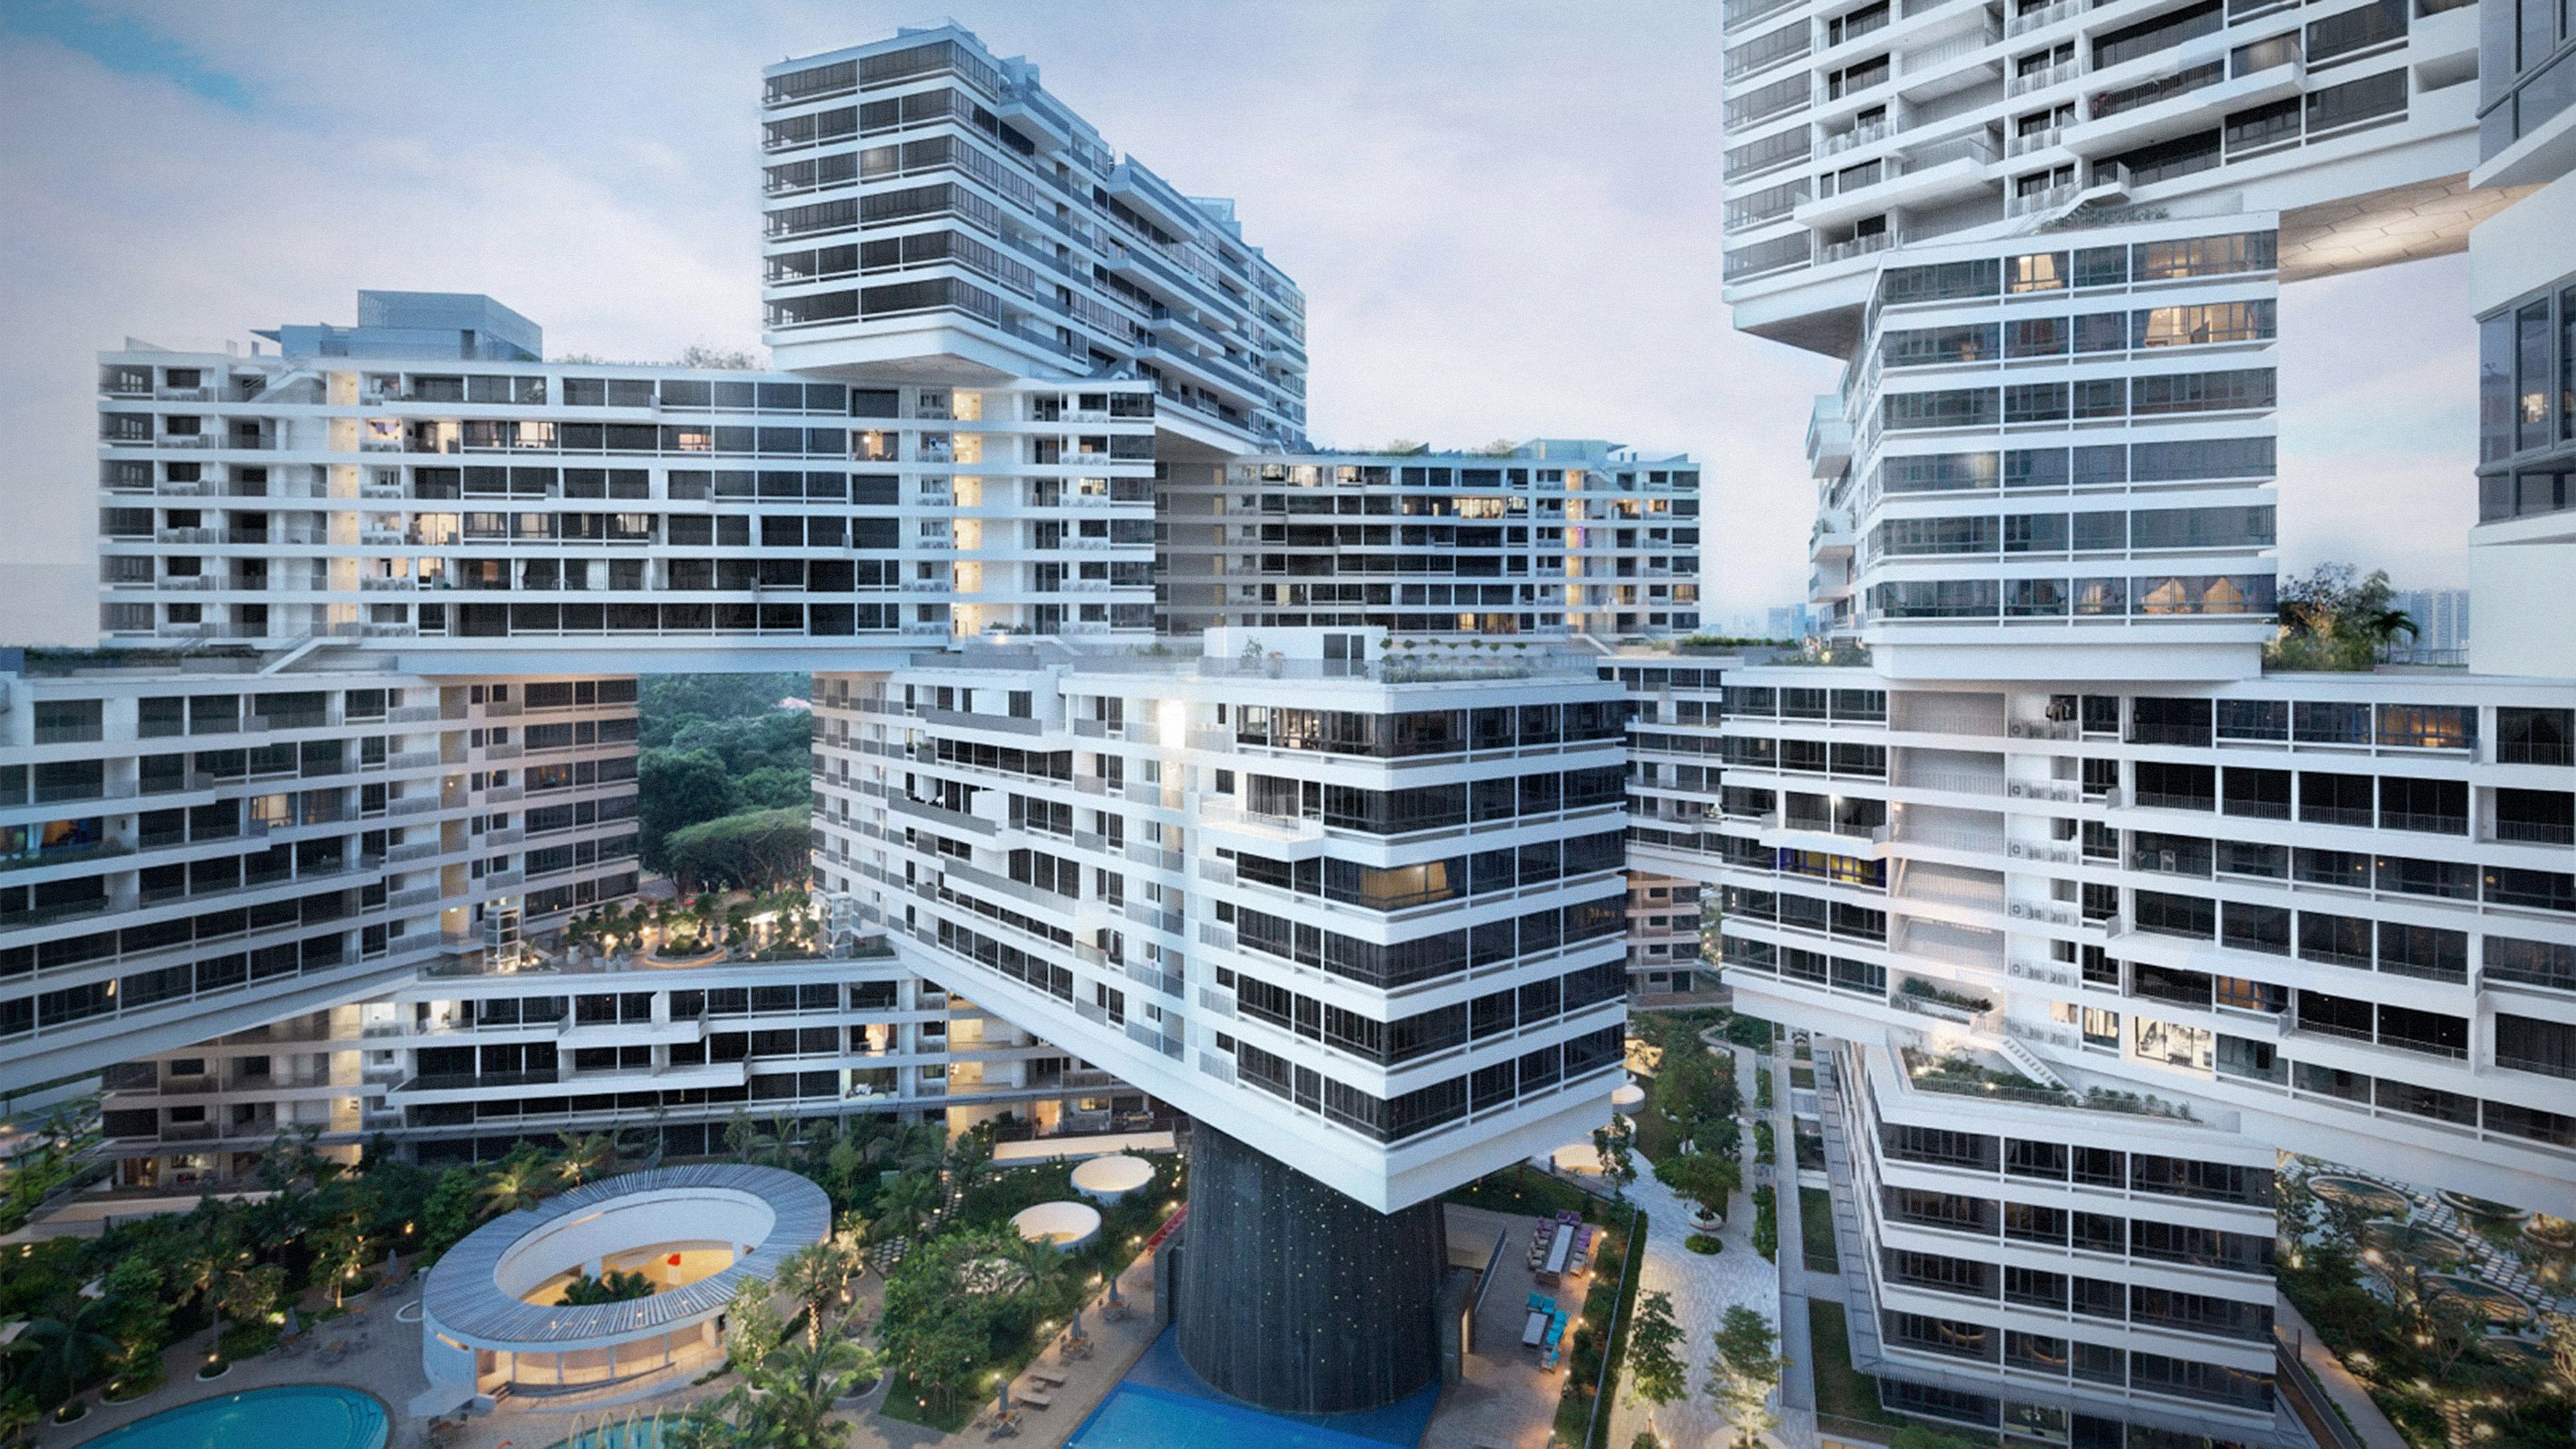
\includegraphics[width=0.3\textwidth]{images/architecture.jpg}
  \begin{itemize}
  \item<2-> Software engineers love architecture principles.
  \item<3-> Who has heard of \emph{design patterns} and the gang of four book?
  \item<4-> The authors were actually inspired by a book that came up with
    a pattern language in architecture
  \item<5-> Such patterns were meant to provide guidelines across buildings in multiple
    style \emph{abstracting} away concrete details of individual buildings.
  \item<6-> Software design patterns are thus all about providing \emph{abstractions}.
  \end{itemize}
\end{frame}

\begin{frame}
  \frametitle{Theories of Abstraction}
  Let's talk about abstraction.
  \begin{itemize}
  \item<2-> 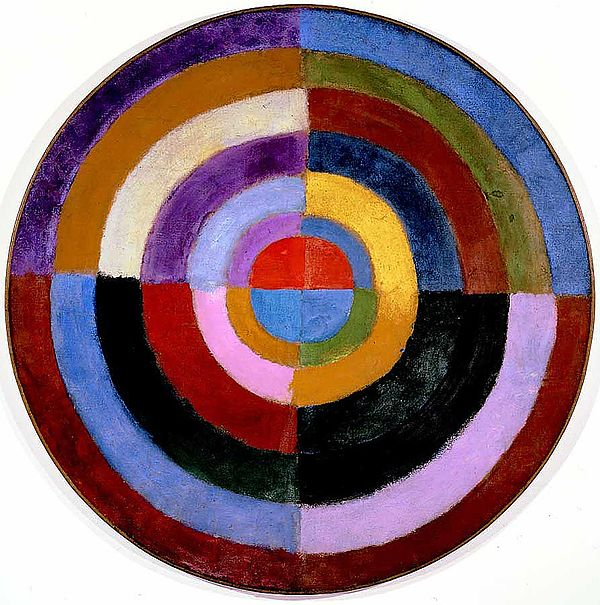
\includegraphics[width=0.3\textwidth]{images/abstract-art.jpg}
  \item<3-> Abstraction in visual
    art is about avoiding concrete subjects. It attempts
    to convey something (often an emotion) without appealing to sentiment.
  \item<4-> Oddly enough there's a bit of a stigma against it, despite the
    fact that music without lyrics has far less stigma.
  \item<5-> Abstraction in mathematics and computer science is about
    \emph{generalization}. Take away the concrete details of certain objects
    and see how they are similar.
  \end{itemize}
\end{frame}

\begin{frame}
  \frametitle{Why Abstract?}
  This can lead us to \emph{classify} different objects into
    related groups.
  \begin{itemize}
  \item<2-> Category theory has been influential in programming language theory
    because it is a powerful language for communicating abstractions in ways
    that are largely \emph{constructive}.
  \item<3-> This is important to computing because the point of programs
    are to construct some form of answer.
  \item<4-> Although categorical abstractions are powerful, I will not discuss them much (and most of the really powerful abstractions go over my head).
  \item<5-> But we will study abstraction from a less mathematical viewpoint.
  \item<6-> I will show instances of \emph{almost identical} code and how a programming language feature allows the two pieces of code to be generalized. 
  \end{itemize}    
\end{frame}

\defverbatim[colored]\buddies{
\begin{minted}[fontsize=\footnotesize]{Java}
  public boolean HasSmith(List<String> names) {
    for (String name : names) {
      if (name == "Smith")
        return true;
    }
    return false;
  }

  public  boolean HasBob(List<String> names) {
    for (String name : names) {
      if (name == "Bob")
        return true;
    }
    return false;
  }
\end{minted}
}

\begin{frame}
  \frametitle{Buddy Functions}
  Let's consider the following functions in Java:
  \buddies
  \pause
  These look pretty similar, right?
\end{frame}

\defverbatim[colored]\abstractOne{
\begin{minted}[fontsize=\footnotesize]{Java}
  public boolean HasName(String searchName, List<String> names) {
    for (String name : names) {
      if (name == searchName)
        return true;
    }
    return false;
  }
\end{minted}
}

\begin{frame}
  \frametitle{Eliminate Redundancy!}
  So, let's eliminate the redundancy of searching
  for different names by abstracting out towards
  a definition that takes in a string parameter
  to search for. This generalizes writing functions
  to search for specific strings.

  \abstractOne
  \begin{itemize}
  \item<2-> Why only design a function that searches for names?
  \item<3-> Why not search for arbitrary items so long as they
    are comparable?
  \item<4-> Then searching for names becomes an instance of a
    more general problem that is solved.    
  \end{itemize}
\end{frame}

\defverbatim[colored]\abstractTwo{
\begin{minted}[fontsize=\footnotesize]{Java}
  public <T extends Comparable<T>>
    boolean HasItem(T searchItem, List<T> items) {
    for (T item : items) {
      if (item.equals(searchItem))
        return true;
    }
    return false;
  }
\end{minted}
}

\begin{frame}
  \frametitle{Generic Structure}
  So, let's use some Java \emph{generics} to generalize our program.
  \abstractTwo
  \begin{itemize}
  \item<2-> Alright, now we can search for arbitrary comparable items!
  \item<3-> This is nice and general!
  \item<4-> Can we generalize any more?
  \item<5-> We actually have 2 more abstractions that we can apply!
  \end{itemize}
\end{frame}

\begin{frame}
  \frametitle{Two Abstractions??}
  \centering 
\includegraphics[width=0.6\textwidth]{images/two-abstractions.jpg}
\end{frame}

\begin{frame}
  \frametitle{I'm Sorry}
  \centering 
\includegraphics[width=0.6\textwidth]{images/unnecessary.png}
\end{frame}

\defverbatim[colored]\abstractThree{
\begin{minted}[fontsize=\footnotesize]{Java}
  public <T extends Comparable<T>>
    boolean TestItems(Predicate<T> pred, List<T> items) {
    for (T item : items) {
      if (pred.test(searchItem))
        return true;
    }
    return false;
  }
\end{minted}
}

\begin{frame}
  \frametitle{Back on Track}
  Ok, let's get down to business.
  \begin{itemize}
  \item<2-> 
\includegraphics[width=0.3\textwidth]{images/business.png}
  \item<3-> We can actually consider searching for a specific item via equality
    as the process of seeing if an arbitrary predicate returns true for an item
    in a list.
  \item<4-> So if we wanted to check if a string equaled smith we could write:
    \mintinline{Java}{Predicate<String> isSmith = str -> str == "Smith";}
  \item<5-> I could then pass this as the first argument to a funciton \mintinline{Java}{TestItems}
    that I will now define.
  \end{itemize}
\end{frame}

\defverbatim[colored]\abstractFour{
\begin{minted}[fontsize=\footnotesize]{Java}
  public <T extends Comparable<T>>
    boolean TestItems(Predicate<T> pred, Iterable<T> items) {
      for (T item : items) {
        if (pred.test(searchItem))
          return true;
      }
      return false;
    }
\end{minted}
}

\begin{frame}
  \frametitle{Last Abstraction}
  Here is that function now:
  \abstractThree
  \begin{itemize}
  \item<2-> We can provide one last abstraction that applies predicates to every item in \emph{any iterable collection}.
  \item<3-> For example, if I define iterators over dictionaries or trees we should still be able to
    apply a predicate to them.
  \item<4-> \abstractFour
  \end{itemize}
\end{frame}

\begin{frame}
  \frametitle{Predicates as Arguments}
  Our third abstraction was a bit strange, right?
  \begin{itemize}
  \item<2-> I used this weird predicate type in Java and then assigned an \emph{anonymous function}.
  \item<3-> This is a function with no name, and it is useful if you only need to use a function
    in one place in your program.
  \item<4-> The second thing is that we had a parameter that received a function as input.
  \item<5-> It then applied this function to every element in the list and observed whether it
    returned \mintinline{Java}{true} for that element.
  \item<6-> This is a very powerful concept where we can determine if perhaps all elements in a collection
    satisfy a property or even one element. Or we can collect all individuals in a collection that satisfy
    some property.
  \item<7-> For example, let's consider writing a program that only admits people that are 18 and older. 
  \end{itemize}
\end{frame}

\defverbatim[colored]\BarEntry{
\begin{minted}[fontsize=\footnotesize]{racket}
  ;; List<Person> -> List<Person>
  ;; Only allows patrons over 18 to enter the bar
  (define (bar-entry patrons)
    (cond
      [(empty? patrons) patrons]
      [(cons? patrons)
         (... (first patrons)) ... (bar-entry (rest patrons))]))  
\end{minted}
}

\begin{frame}
  \frametitle{Guarding Entry}
  Let's consider that we have a list of people whose ages are represented by Natural numbers and that we want to only collect the people
  over 18. Assume a person has an age field that we can project.
  \begin{itemize}
  \item<2-> How do we start writing such a function?
  \item<3-> Via recursion over a list of course.
  \item<4-> I'll skip to providing a skeleton:
  \item<5-> \BarEntry
  \end{itemize}
\end{frame}

\begin{frame}
  \frametitle{Guarding Entry}
  So, in order to protect against underage patrons getting in, we must do a comparision.
  \begin{itemize}
  \item<2-> Assume that \mintinline{racket}{(first patrons)} returns \mintinline{racket}{(person "Sara" 26)}.
  \item<3-> How do I get the age out?
  \item<4-> \mintinline{racket}{(person-age (first patrons))}
  \item<5-> How do I check whether the age is less than 18?
  \item<6-> \mintinline{racket}{(< (person-age (first patrons)) 18)}
  \item<7-> Thus, we should get \mintinline{racket}{(< 26 18)} since we are getting Sara as our person,
    and this should return false.
  \item<8-> Since this returns false, we should throw Sara into the list we're building. How do we do that?
  \item<9-> With \mintinline{racket}{(cons (first patrons) ...)}  
  \end{itemize}
\end{frame}

\begin{frame}
  \frametitle{Only Collecting \emph{Some} Items}
  But what if \mintinline{racket}{(first patrons)} returns \mintinline{racket}{(person "Dustin" 16)}?
  \begin{itemize}
  \item<2-> Then, we had \mintinline{racket}{(< (person-age (person "Dustin" 16)) 18)}
  \item<3-> which evaluates to \mintinline{racket}{(< 16 18)} and then return true.
  \item<4-> This means that we must not add Dustin to our patron list. So we shouldn't use a cons operation.
  \item<5-> There are two ways around this. One is to locally add a complicated if expression. The second is to design
    a new function that only does a cons operation if the first element of the list has an age greater than 18 and otherwise
    returns the sublist that already had filtered out underage people.
  \item<6-> Let's consider designing this second function, called \mintinline{racket}{cons-over-18}
  \item<7-> Does this function need to do recursion itself?
  \end{itemize}
\end{frame}

\defverbatim[colored]\ConsOver{
\begin{minted}[fontsize=\footnotesize]{racket}
    ;; List<person> -> List<person>
    ;; Add a person to the patron list as
    ;; long as they are over 18.
    (define (cons-over-18 possible-patron patrons)
      (if (>= (person-age possible-patron) 18)
          (cons possible-patron patrons)
          patrons))  
\end{minted}
}

\begin{frame}
  \frametitle{Designing a Helper Function}
  Thankfully, our helper function does not need to do recursion!
  \begin{itemize}
  \item<2-> Why?
  \item<3-> We assume that the recursion for \mintinline{racket}{bar-entry} already filters out people from sublists.
  \item<4-> So, our helper function simply takes in a person and a list
    and only conses the person onto the list if they are over 18.
  \item<5-> \ConsOver
  \end{itemize}
\end{frame}

\defverbatim[colored]\BarFinal{
\begin{minted}[fontsize=\footnotesize]{racket}
  ;; List<Person> -> List<Person>
  ;; Only allows patrons over 18 to enter the bar
  (define (bar-entry patrons)
    (cond
      [(empty? patrons) patrons]
      [(cons? patrons)
         (cons-over-18 (first patrons) (bar-entry (rest patrons)))]))    
\end{minted}
}

\begin{frame}
  \frametitle{Finishing Our Bouncer Program}
  Alright, with our helper combinator we can structure our recursive function
  in the usual way, instead of having to add an additional condition in the
  body of the function.
  \begin{itemize}
  \item<2-> \BarFinal
  \item<3-> In general, if it seems like the list you're building depends
    on the structure of the values in the list, then you need some kind
    of cons operation that checks properties on the head of the list.
  \item<4-> But what happens if the condition we are checking needs to change?
  \end{itemize}
\end{frame}

\defverbatim[colored]\BarComplex{
  \begin{minted}[fontsize=\footnotesize]{racket}
    (define (cons-over-18 possible-patron patrons)
      (if (>= (person-age possible-patron) 18)
          (cons possible-patron patrons)
          patrons))
    (define (bar-entry-18 patrons)
      (cond
        [(empty? patrons) patrons]
        [(cons? patrons) (cons-over-18
                           (first patrons)
                           (bar-entry-18 (rest patrons)))]))
    (define (cons-over-21 possible-patron patrons)
      (if (>= (person-age possible-patron) 21)
           (cons possible-patron patrons)
           patrons))
    (define (bar-entry-21 patrons)
      (cond
        [(empty? patrons) patrons]
        [(cons? patrons) (cons-over-21
                          (first patrons)
                          (bar-entry-21 (rest patrons)))]))
  \end{minted}
}

\begin{frame}
  \frametitle{Adjusting Our Bouncer Program}
  Concretely, let's say that that our bar was serving alcohol to
    patrons under 21 (this is illegal but common...) and a new Sheriff comes in
    and is stricter on enforcing alcohol laws.
    \begin{itemize}
  \item<2-> Now our bar can't afford to give drinks to patrons under 21 years old.
    We decide that the easiest solution is to only allow 21 and over patrons,
    to prevent underage people from getting in and sneakily get drinks.
  \item<3-> To model this behavior, our program must change
    \mintinline{racket}{cons-over-18} to something named \mintinline{racket}{cons-over-21} that changes its check to make sure patrons are at least 21.
  \item<4-> But let's say we still need to model another bar that allows people over 18, but charges them covers. Then we will need four functions for our program.  
  \end{itemize}
\end{frame}

\begin{frame}
  \frametitle{Repetitive Bar Program}
  \BarComplex
\end{frame}

\begin{frame}
  \frametitle{How to Eliminate Redundant Code}
  So, we can see we have a lot of redundant code in the program.
  \begin{itemize}
  \item<2-> Redundant code should cause developers an itch.
  \item<3-> On the one hand, there are more places for the program
    to go wrong.
  \item<4-> On the other, most developers get bored of re-reading similar code.
  \item<5-> To minimize failure locations and keep interest, we should
    \emph{abstract} out patterns in the code.
  \item<6-> So, how do we get started?
  \end{itemize}
\end{frame}
\end{document}
%%% Local Variables:
%%% TeX-command-extra-options: "-shell-escape"
%%% mode: latex
%%% TeX-master: t
%%% End:
